\section{ХОД РАБОТЫ}

\subsection{Постановка задачи}

Необходимо написать валидатор XML-документов с графическим интерфейсом.

\subsection{Особенности разработанного приложения}

Разработанное приложение представляет собой типичное графическое
приложение, написанное с использованием GTK, а также класса XML-валидации,
приведенного в разделе~\ref{sec:theory}.

На рисунке~\ref{pic:interface} приведен пользовательский интерфейс
разработанного приложения.

\begin{figure}[h!]
  \centering
  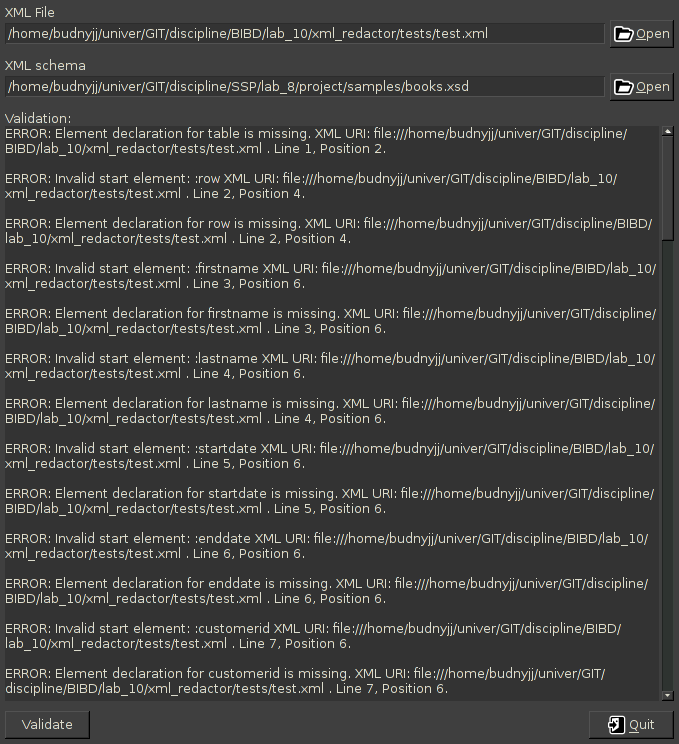
\includegraphics[width=92mm]{pic/interface}
  \caption{Интерфейс разработанного приложения}
  \label{pic:interface}
\end{figure}

Исходный текст разработанного приложения находится в приложении~А.